\chapter{Ход работы}
\label{ch:chap2}

\section*{\textbf{Моделирование цепи Маркова. Визуализация переходов}}

Для лабораторной работы используется матрица переходов из лабораторной работы №1. Вот так выглядит цепь Маркова для такой матрицы
переходов:

\begin{figure}[H]
    \centering
    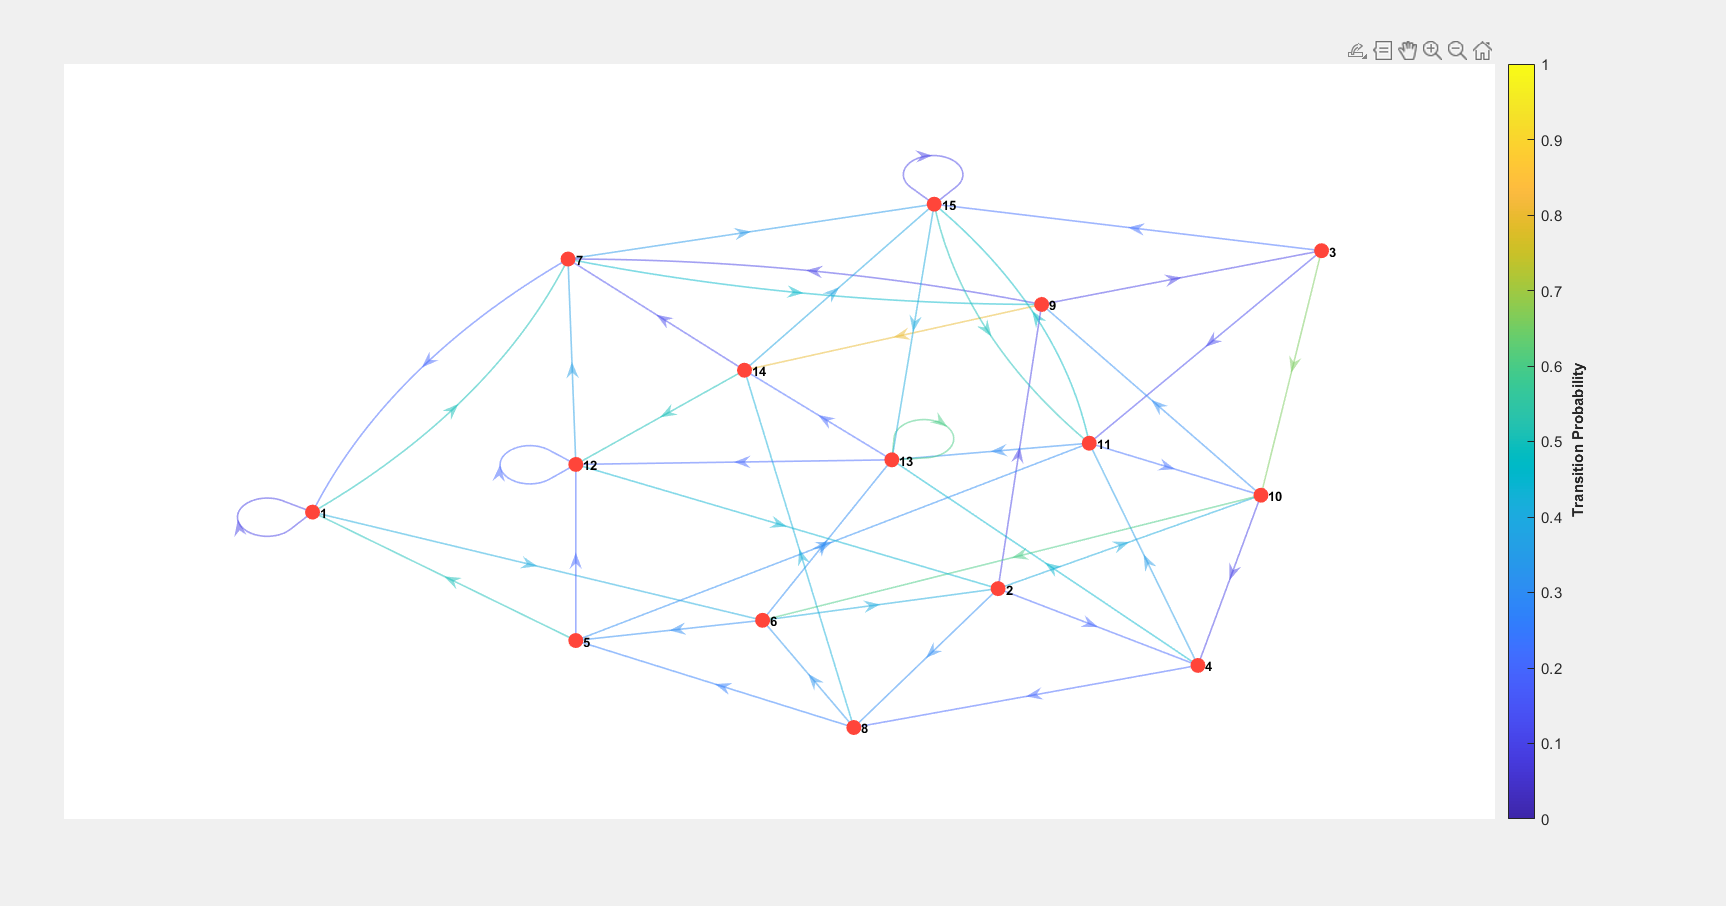
\includegraphics[width=1.0\textwidth]{chain.png}
    \caption{Цепь Маркова. L=15}
\end{figure}

С помощью функции, данной в теории, промоделируем цепь Макрова, т.е посомтрим, как будут осуществляться переходы между состояниями.
Для этого зададим функцию:

\begin{lstlisting}
function E = MarkovTrajectory(P, N, s)        
        E = zeros(1, N + 1);
        E(1) = s;  
        S = size(P, 1); 
        
        for i = 1:N
        r = rand();
        cumulativeProb = 0;
        
        for j = 1:S
            cumulativeProb = cumulativeProb + P(E(i), j);
            if r < cumulativeProb
                E(i + 1) = j;
                break;
            end
        end
    end
end
\end{lstlisting}

А потом вызовем ее в коде и получим вектор, содержащий состояния цепи Маркова в каждый момент времени, и построим график переходов.

\begin{lstlisting}
%modeling markov chain
N = 400;
start = 1;
E = MarkovTrajectory(P, N, start);

%create and show plot
t = 0 : 1 : N;

figure;
plot(t, E);
\end{lstlisting}

\begin{figure}[H]
    \centering
    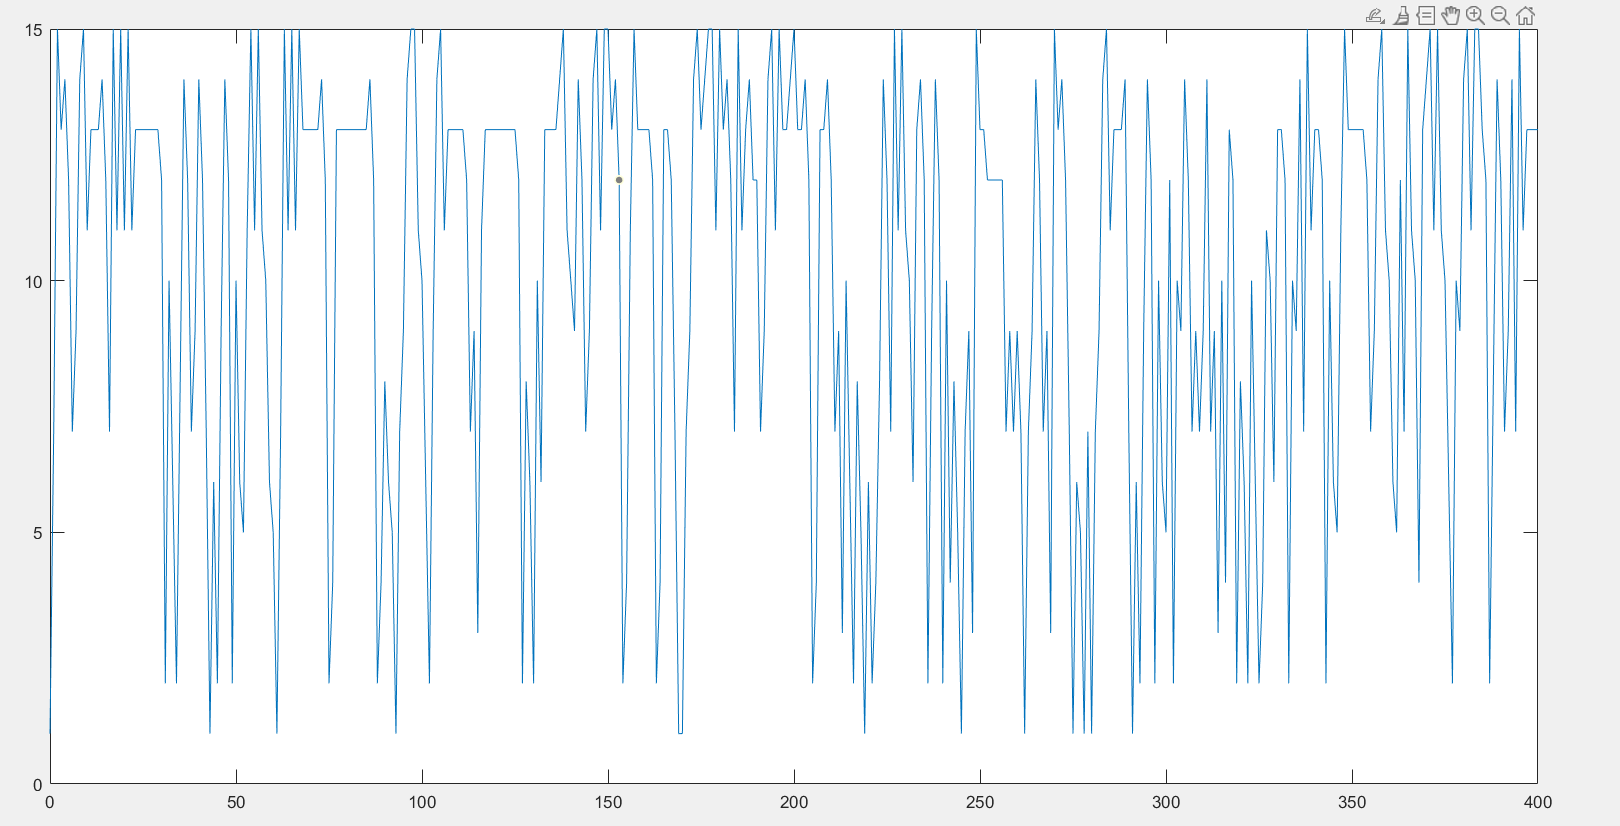
\includegraphics[width=1.0\textwidth]{modelation.png}
    \caption{График переходов между состояними в цепи Маркова}
\end{figure}

Можем наблюдать случайный процесс.

\section*{\textbf{Вычислим вероятность пребывания пакета в узле j после m коммутаций, при условии, что пакет поступил в сеть через узел i}}

Для этого необходимо возвести матрицу переходов P в степень m и взять элемент $P_{ij}$. Почему матрица возводится в степень?
Дело в том, что матрица умноженная саму на себя дает все комбинации переходов. Если просчитывать все комбинации отдельно, то в 
конечном счете получим матричное умножение P саму на себя. \\

Реализация функции:

\begin{lstlisting}
function P_ij = func_1(P, m, i, j)
    Pm = P^m;         
    P_ij = Pm(i, j); 
end
\end{lstlisting}

Найдем вероятность перехода из состояния 2 в состояние 4 за 2 шага и выведем результат:

\begin{lstlisting}
P_ij = func_1(P, 2, 2, 4);
disp(P_ij);
\end{lstlisting}

В результате получим 0.04. Если анализировать граф, то можно заметить, что такая ситуация может быть только при переходах 2->10->4.
Вероятность перейти из 2 в 10 составляет 0.4, а перейти из 10 в 4 - 0.1. 0.4 * 0.1 = 0.04. Значит, все верно.

\section*{\textbf{Вычислим вероятность первого перехода пакета в узел j из узла i после m коммутаций}}

Иными словами, m-1 шагов мы не попадали в узел j, а на шаге m попали. Т.е нам нужно на каждом m-1 шаге перемножать вероятность
НЕ попасть в нужный узел с вероятностью попасть в узел на шаге m.

Реализация:

\begin{lstlisting}
function res = func_2(P, m, i, j)
    k = 0;
    cum_mul = 1;
    P_tmp = P;
    while k < m - 1
        cum_mul = cum_mul * (1 - P_tmp(i,j));
        P_tmp = P_tmp * P; 
        k = k + 1;
    end
    if m > 1
         P_tmp = P_tmp * P;
    end
   
    res = P_tmp(i,j) * cum_mul;
end

\end{lstlisting}

Найдем вероятность первого перехода из состояния 2 в состояние 4 за 4 шага и выведем результат:

\begin{lstlisting}
P_m2 = func_2(P, 4, 2, 4);
disp(P_m2);
\end{lstlisting}

Получаем 0.142

\section*{\textbf{Вычислим длину кратчайшего пути перехода пакета в узел j из узла i}}

Логично, что кратчайший путь - минимальное m, при котором  $P_{ij} != 0$. То есть необходимо перемножать матрицу на себя до тех
пор, пока не найдется такое m. Если в графе одна компонента сильной связности (нет изолированной точки), то такое значение обязательно
существует. \\

Реализация:


\begin{lstlisting}
function res = min_len(P, i, j)
    m = 1;
    while P(i,j) == 0
        P = P * P; 
        m = m + 1;
    end
    res = m;
end
\end{lstlisting}

Рассчитаем минимальный путь из узла 2 в узел 13:

\begin{lstlisting}
min_l = min_len(P, 2, 13);
disp(min_l);
\end{lstlisting}

В результате получаем 2, что логично, ведь есть маршрут 2->4->13.

\section*{\textbf{Вычислим математическое ожидание длины пути перехода пакета в узел j из узла i}}

Для вычисление мат.ожидания необходимо на каждом шаге коммутации умножать m (длину пути) на вероятность первого пребывания в узле
$P_{ij}$. По сути это стандартное определение мат.ожидания. В идеале вычисления нужно производить бесконечно, чтобы получить
максимально точный результат. Я выставил максимальное число переходов равным 500. Этого вполне хватает, чтобы мат.ожидание сошлось
к какому-то значению. \\

Реализация:

\begin{lstlisting}
function res = m(P, i, j)
    m = 1;
    max_m = 500;
    res = 0;
    while m <= max_m
        f = func_2(P, m, i, j);
        res = res + m * f;
        m = m + 1;
    end
end
\end{lstlisting}

Вычислим мат.ожидание для пути 2->13:

\begin{lstlisting}
E_m = m(P, 2, 13);
disp(E_m);
\end{lstlisting}

Получаем значение 6.8, т.е нам понадобится в среднем 7 ходов, чтобы попасть из узла 2 в узел 13 при минимальной длине пути равной 2.

\section*{\textbf{Вычислим дисперсию длины пути перехода пакета в узел j из узла i}}

Для вычисления необходимо просуммировать шаг коммутации в квадрате, умноженный вероятность первого пребывания пакета в узле. Потом
от этой суммы нужно отнять мат.ожидание длины пути в квадрате. По сути тоже стандарное определение дисперсии. Максимальное значение
m выставил равным 500. \\

Реализация:

\begin{lstlisting}
function res = D(P, i, j)
    m = 1;
    max_m = 500;
    res = 0;
    while m <= max_m
        f = func_2(P, m, i, j);
        res = res + m^2 * f;
        m = m + 1;
    end

    res = res - M(P, i, j)^2;
end
\end{lstlisting}

Вычислим дисперсию для пути из узла 2 в узел 13:
\begin{lstlisting}
D_E = D(P, 2, 13);
disp(D_E);
\end{lstlisting}

Получим 15.7. Это значит, что длина маршрута может отклоняться от средней длины на $+-\sqrt{15.7} \approx 3.9$ шагов. \\

\section*{\textbf{Графики}}

Построим графики зависимости вычисленных характеристик от номеров узлов.

\begin{figure}[H]
    \centering
    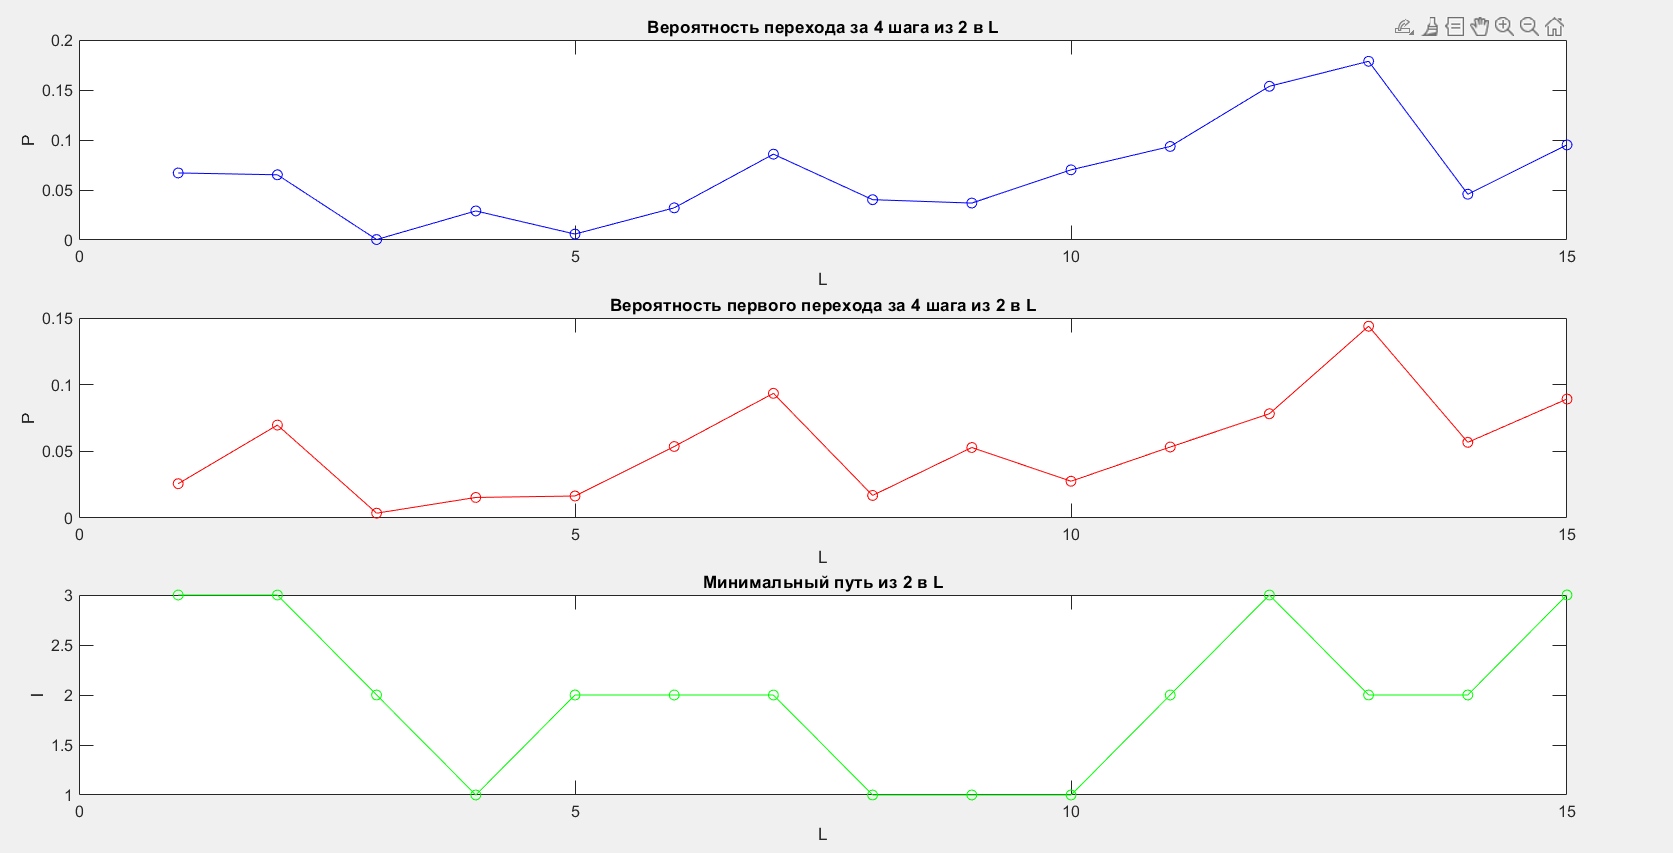
\includegraphics[width=1.0\textwidth]{plot1.png}
    \caption{При i = 2, j = [1,16]}
\end{figure}

\begin{figure}[H]
    \centering
    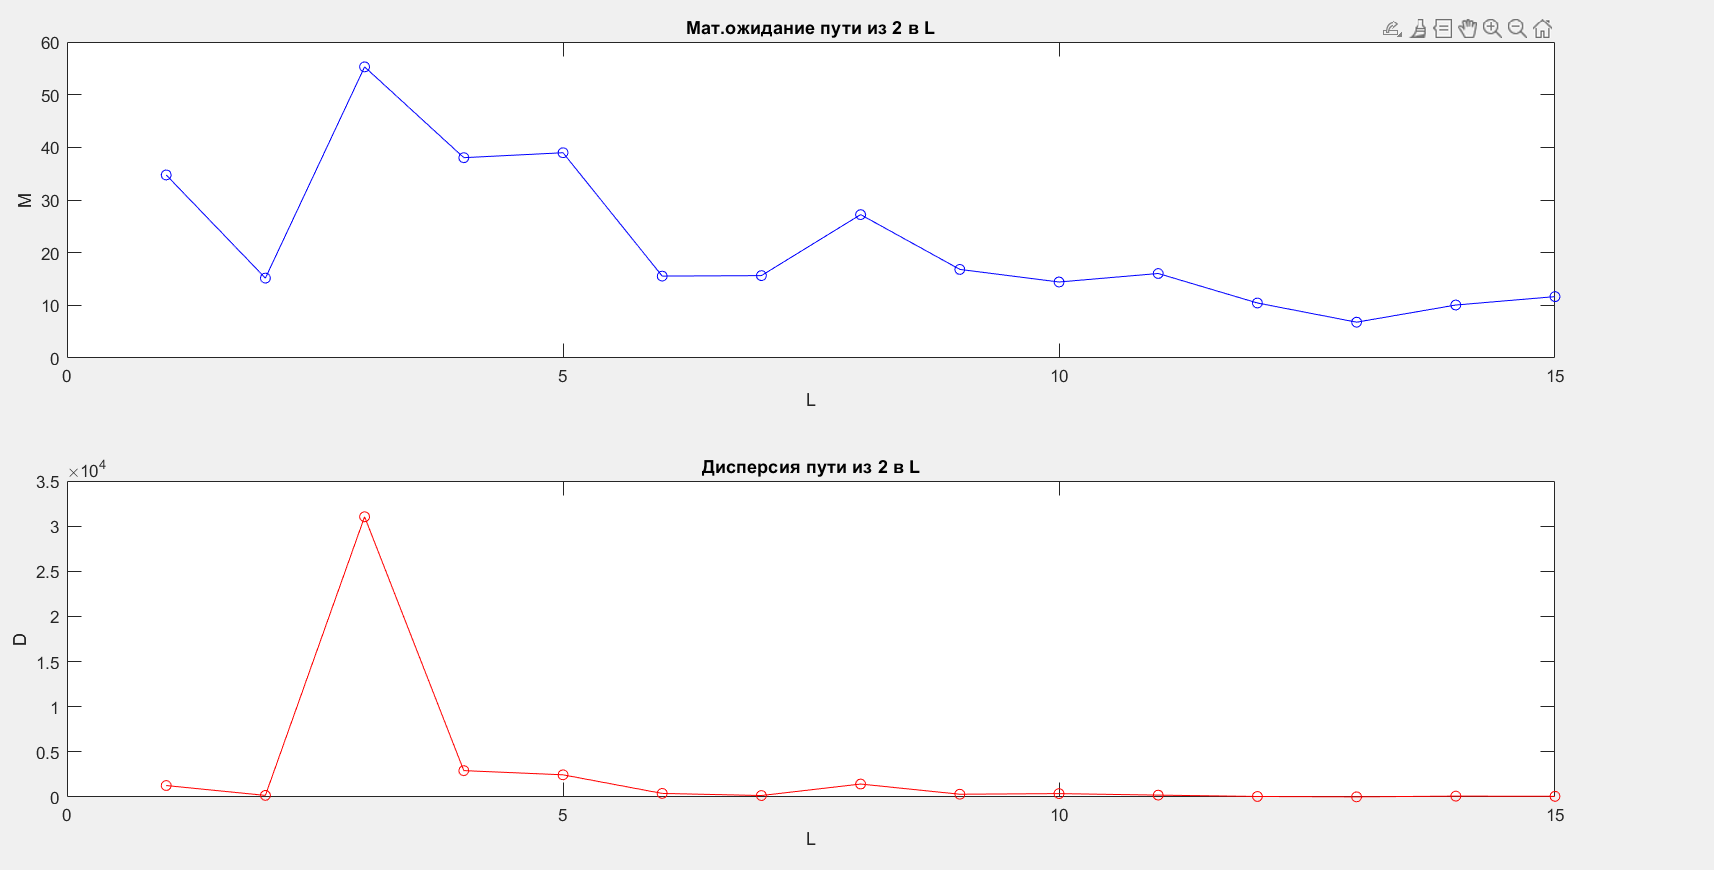
\includegraphics[width=1.0\textwidth]{plot2.png}
    \caption{При i = 2, j = [1,16]}
\end{figure}

Можем заметить, что какой-то взаимосвязи между номерами узлов и характеристиками нет. Характеристики ведут себя случайно. Влияние
оказывает скорее сама матрица переходов и кол-во переходов m (в функциях, где она нужна). Может, я неудачно подобрал номера узлов?
Построим графики при i = 13 и переменных j:

\begin{figure}[H]
    \centering
    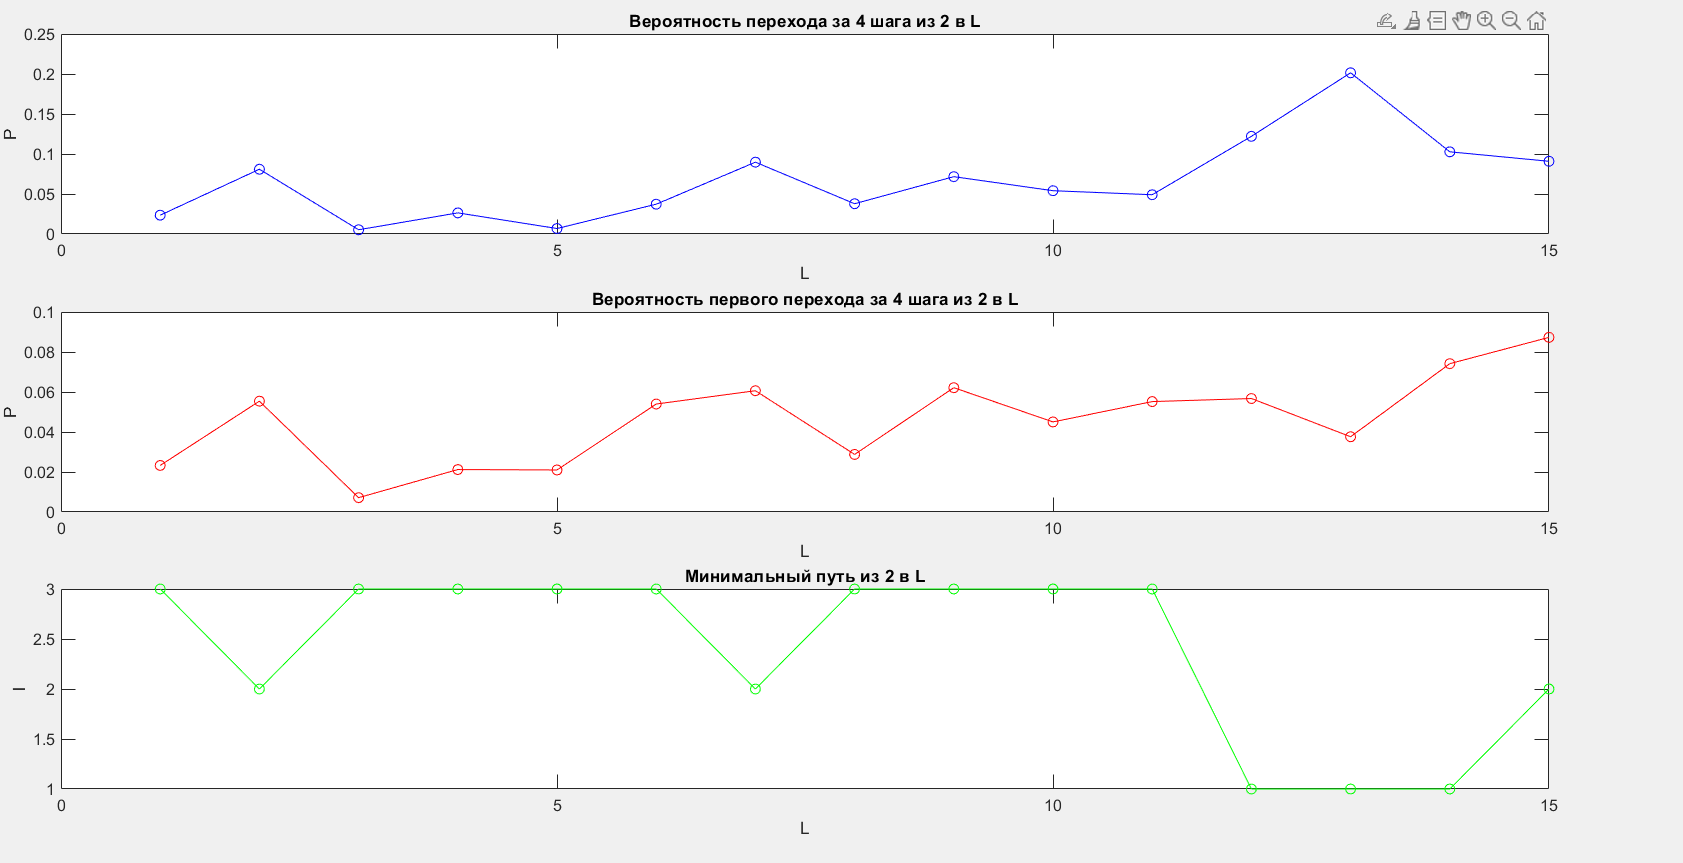
\includegraphics[width=1.0\textwidth]{plot1_13.png}
    \caption{При i = 13, j = [1,16]}
\end{figure}

\begin{figure}[H]
    \centering
    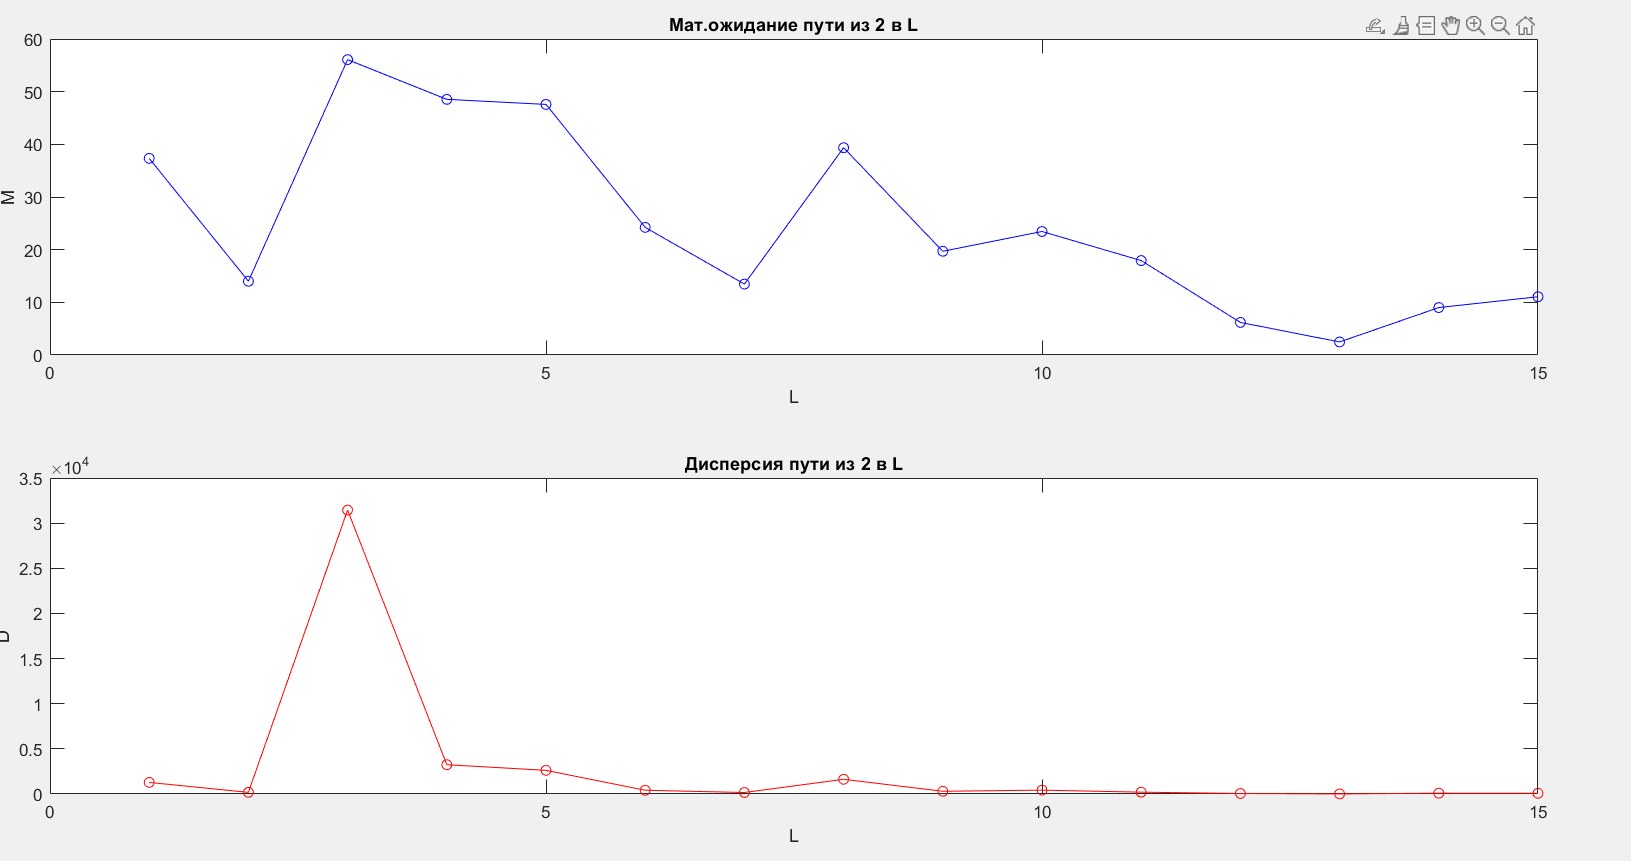
\includegraphics[width=1.0\textwidth]{plot_2_13.png}
    \caption{При i = 13, j = [1,16]}
\end{figure}

Видим, что зависимости тоже нет, но ведут себя графики очень похоже. Это значит, что нет разницы, в какой точке пакет входит в сеть
и в какую точку его необходимо доставить. На это влияют другие характеристики.

\section*{\textbf{Контрольные вопросы}}

\begin{figure}[H]
    \centering
    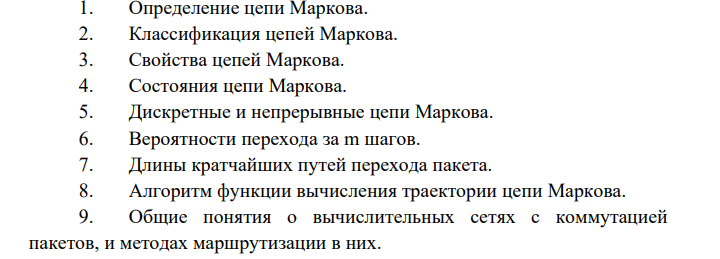
\includegraphics[width=1.0\textwidth]{question.png}
    \caption{Контрольные вопросы к лабораторной работе}
\end{figure}

\begin{enumerate}
    \item 1.Цепь Маркова – последовательность случайных событий с конечным или счётным числом исходов, характеризующаяся тем 
    свойством, что, говоря нестрого, при фиксированном настоящем будущее независимо от прошлого.
    \item 2. Цепи Маркова бывают однородные, т.е при шагах коммутации матрица переходов не изменяется (не зависит от шагов и времени).
    Также цепи Маркова бывают стационарные, т.е если цепь задана каким-то распределением, то это распределение остается неизменным.
    Неприводимая цепь Маркова - цепь Маркова, в которой из любого состояние можно попасть в любое другое за конечное число шагов.
    Эргодичная цепь Маркова - цепь Маркова, которая сходится к какому-то распределению.
    \item 3. Состояния цепи Маркова - позиции, в которых может находиться система. Также это вершины графа.
    \item 4. Дискретные цепи Маркова определены только в дискретные моменты времени (k = 0,1,2...). Непрерывные цепи Маркова
    определены в любой момент времени из области определения. Они обладают разными параметрами.
    \item 5. Вероятность перехода за m шагов коммутации - это та вероятность, с которой система окажется в состоянии N за m шагов.
    На каждом шаге коммутации матрица перемножается сама на себя, таким образом просчитываются все возможные комбинации (переходы).
    \item 6. Длины кратчайших путей перехода пакета - минимальное число переходов для перехода из состояния i в состояние j.
    Вычисляется путем подбора такого m (шагов коммутации) при котором  $P_{ij}$ != 0.
    \item 7. Алгоритм функции вычисления траектории цепи Маркова заключается в том, что в каждый дискретный момент времени вычисляется
    случайное число на отрезка [0;1] по равномерному распределнию и потом нужно подобрать такое следующее состояние системы k, при котором
    сгенерированное число будет меньше, чем вероятность перехода в состояние k. Это симулирует случайность при переходах.
    \item 8. Сеть с коммутацией пакетов - сеть, в которой данные передаются не потоком, а пакетами, содержащими полезную нагрузку
    и служебную информацию. Основные методы маршрутизации RIP, OSPF, BGP, MPLS, Static Route. 

\end{enumerate}

\endinput
